% INTERCEPT submission skeleton: Judgment-Layer Drift, No Changelog
%
% Prose mirrors paper/INTERCEPT_DRAFT.md (2026-08-22 draft, updated
% 2026-08-23) verbatim, with only mechanical conversion:
%   - [FREEZE: ...] tags render through \freeze{...} in red; every one
%     is a placeholder to swap at the 2026-09-26 data freeze. Do not
%     hand-edit a red number without a script behind it.
%   - Numeric cross-references (3.1.1, 3.3, T1) became \ref{} labels.
%   - Citation brackets ([casper, cai]) became \cite{} keys; the
%     bibliography is references.bib, IEEEtran.bst style. Entries
%     marked TODO await the pre-submission citation pass.
%   - Scientific notation typeset ($5.5\times10^{-5}$ for 5.5e-5).
%   - Figure/table callouts (Fig.~1 etc.) added; the draft implies
%     placement but never cites figures inline.
%   - The section 7 blind-review bracket renders as a blue PENDING
%     note via \pendingnote{...}; decision open per the handoff.
% Anonymity: \anonymoustrue below until the blind-review decision is
% made (docs/claude_code_handoff_intercept_paper.md, Blind-review
% handling). Flip to \anonymousfalse for camera-ready.
% Build: ./build.sh (pdflatex + bibtex; IEEEtran.cls/.bst vendored
% here so the build needs no publisher package installed).
% Venue: INTERCEPT Defenders track, IEEE conference PDF under 4 MB,
% 4 to 6 pages, submission closes 2026-10-01.

\documentclass[conference]{IEEEtran}

\usepackage{graphicx}
\usepackage{xcolor}
\usepackage{url}
\usepackage{amsmath}

\graphicspath{{../figures/out/}}

% Freeze placeholders: red and impossible to miss until the swap.
\newcommand{\freeze}[1]{\textcolor{red}{[FREEZE: #1]}}
\newcommand{\freezebare}{\textcolor{red}{[FREEZE]}}
% Editorial decisions still open at drafting time.
\newcommand{\pendingnote}[1]{\textcolor{blue}{[PENDING: #1]}}

\newif\ifanonymous
\anonymoustrue % blind-review decision pending; see header comment

\begin{document}

\title{Judgment-Layer Drift, No Changelog:\\
\freeze{55} Days Monitoring Five LLM APIs}

\ifanonymous
\author{\IEEEauthorblockN{Anonymous submission}
\IEEEauthorblockA{INTERCEPT Defenders track}}
\else
\author{\IEEEauthorblockN{Anna Hix}
\IEEEauthorblockA{hix.anna@gmail.com}}
\fi

\maketitle

\begin{abstract}
Served LLM behavior changes behind stable model ids, and the change
has a shape. I ran a calibrated behavioral monitor against five
production LLM APIs daily for \freeze{55} days: a frozen 68-item
security judgment bank, $K=10$ samples per item, per-item total
variation distance against a frozen baseline, simulation-calibrated
alarm bands, and a same-day disambiguation rerun on every breach.
Three findings. First, judgment behavior oscillates: models revisit
exact prior answer distributions on contested items, day-scale
dwell, week-scale persistence of the attractor states, entries
sometimes arriving as same-day joint moves across items
(\freezebare{} two round trips in seven days on one vendor). Second,
the movement concentrates entirely where judgment is contested:
\freeze{29 of 29} breach entries landed on designed-equipoise items
while the decisive class produced zero exceedances in \freeze{2,700}
slot-day checks, and quiet equipoise slots show no movement beyond
exact sampling expectation on any vendor: the drift is not ambient,
it lives in named recurring threads. Third, every serving covariate
observable from outside the API stayed constant across
\freeze{41,090} rows while behavior moved, so a customer can detect
the change but cannot attribute it. A snapshot evaluation certifies
the day it ran, not the period it is cited for. The monitor costs
about 20 USD per month, and the full instrument, record, and
analysis are reproducible from a public artifact.
\end{abstract}

% Proposed keywords (not in the prose draft); edit or drop freely.
\begin{IEEEkeywords}
LLM APIs, behavioral monitoring, drift detection, runtime security,
model assurance
\end{IEEEkeywords}

\section{Introduction}

An agent pipeline is qualified against the model serving it.
Nothing announces when that stops being true. Vendors change
weights, quantization, serving configuration, and safety layers
behind stable model ids; the response schema carries no version for
any of it. A control validated last quarter is not validated today,
and no signal reports the expiration.

The gap is not hypothetical. One vendor's published postmortem
documents three concurrent serving-stack bugs, sticky per-user,
missed by the vendor's own evaluations and resolved by rollback
\cite{anthropic-postmortem}. That is the vendor telling us what the
serving layer does when nobody is measuring from outside.

Here is what measuring from outside looks like. On August 2, 2026,
I baselined five production APIs on a 68-item judgment bank and
probed the full bank hours later: 340 slots, zero breaches, every
model clean. The next scheduled probe, one day later, found one
model in a different regime: two items flipped to a joint state
they had occupied three days before, at probabilities on the order
of $10^{-9}$ to $10^{-13}$ under the fresh baseline. The state held
for the same-day rerun, reverted days later, and returned again.
This is not an outage and it is not noise. It is a served model
revisiting a prior behavioral state, on a pinned id, with no
changelog entry.

This paper contributes:
\begin{enumerate}
\renewcommand{\theenumi}{\alph{enumi}}
\renewcommand{\labelenumi}{(\theenumi)}
\item the first documentation, to my knowledge, of reversible
  day-scale regime oscillation in served LLM judgment behavior,
  with exact recurrence of prior answer distributions;
\item a drift instrument built from a stratified judgment bank,
  designed-equipoise items alongside decisive ones, with a
  \freeze{2,700} slot-day zero-movement null on the decisive class;
\item detection-without-attribution measured jointly: behavior
  moved while every observable covariate held;
\item per-vendor temporal phenotypes on two axes, per-call
  commitment and drift morphology: quiet slots show zero excess
  movement on all five models, and drift, where it occurs, is
  discrete unidirectional oscillation or diffuse wander;
\item the instrument itself: reproducible, vendor-agnostic, roughly
  20 USD per month to operate.
\end{enumerate}

\section{Instrument}

The bank is 68 forced-choice enterprise security judgment items,
four options each: 45 decisive items with a derivable best answer
and 23 designed-equipoise items authored to sit near a decision
boundary. Five production models, one pinned arm each, $K=10$
samples per item, daily at 13:00 UTC. The 340 model-item slots each
carry a frozen baseline ($n=20$: two pooled same-day $K=10$ runs)
and a per-item alarm band: the p99 of TVD-to-baseline under a
Laplace-smoothed multinomial simulation, seeds deterministic and
recorded. Bands across the 340 slots: 0.40 $\times$311,
0.45 $\times$28, 0.50 $\times$1
(Table~\ref{tab:instrument}).

A day's probe compares each slot's observed distribution to its
baseline. A breach (strict inequality above band) fires a same-day
rerun of the breached items only, and the rerun disambiguates: a
rerun matching the probe and not the baseline is an EVENT, matching
the baseline back is TRANSIENT, matching neither is UNSTABLE. Every
response row records the echoed model id; a mid-run id change halts
collection for that model (ECHO\_CHANGE). One verdict line per
model per day, appended to a committed log. The verdict grammar is
CLEAN, EVENT, TRANSIENT, UNSTABLE, ECHO\_CHANGE, ERROR, and the
reporting commitment was declared before the first scheduled
observation: quiet windows get published with the same care as
event windows.

The false-alarm rate is not assumed from the band percentile. It is
computed by exact enumeration over all 286 compositions of ten
draws into four options, per item, against each item's band: 1.64
expected false breaches per day if the smoothed baseline is truth,
0.05 if the empirical baseline is truth. Observed daily breach
counts sit against that null throughout
(Fig.~\ref{fig:falsealarm}). Everything above is regenerable from
the committed repository: baselines, bands, seeds, verdict log, and
the enumeration script.

\begin{table}[t]
\caption{Instrument summary.
\freeze{placeholder render, record row reflects data through
2026-08-20; regenerate at the data freeze}}
\label{tab:instrument}
\centering
\small
\begin{tabular}{lp{0.55\columnwidth}}
\hline
parameter & value \\
\hline
item bank & 68 forced-choice judgment items (45 decisive, 23
  designed-equipoise) \\
models & 5 production APIs, one pinned arm each \\
alarm slots & 340 (115 equipoise), zero sentinels \\
cadence & daily, 13:00 UTC, $K=10$ samples per item \\
baseline & frozen $n=20$ per slot (two pooled same-day $K=10$
  runs, 2026-08-02) \\
alarm bands (p99) & 0.40 $\times$311, 0.45 $\times$28,
  0.50 $\times$1 \\
breach test & per-item TVD vs baseline, strictly above band;
  same-day rerun disambiguates \\
verdict grammar & CLEAN, EVENT, TRANSIENT, UNSTABLE,
  ECHO\_CHANGE, ERROR \\
expected false breaches & 1.64/day (smoothed truth), 0.05/day
  (empirical truth), exact enumeration \\
record to date & \freeze{19 probe days, 60,270 calls} \\
operating cost & about 20 USD per month \\
\hline
\end{tabular}
\end{table}

\section{Findings}

\subsection{Regime oscillation with exact recurrence}
\label{sec:oscillation}

The headline behavior is not drift in the gradual sense. It is
discrete states, revisited exactly (Fig.~\ref{fig:regime}).

\begin{figure}[t]
\centering
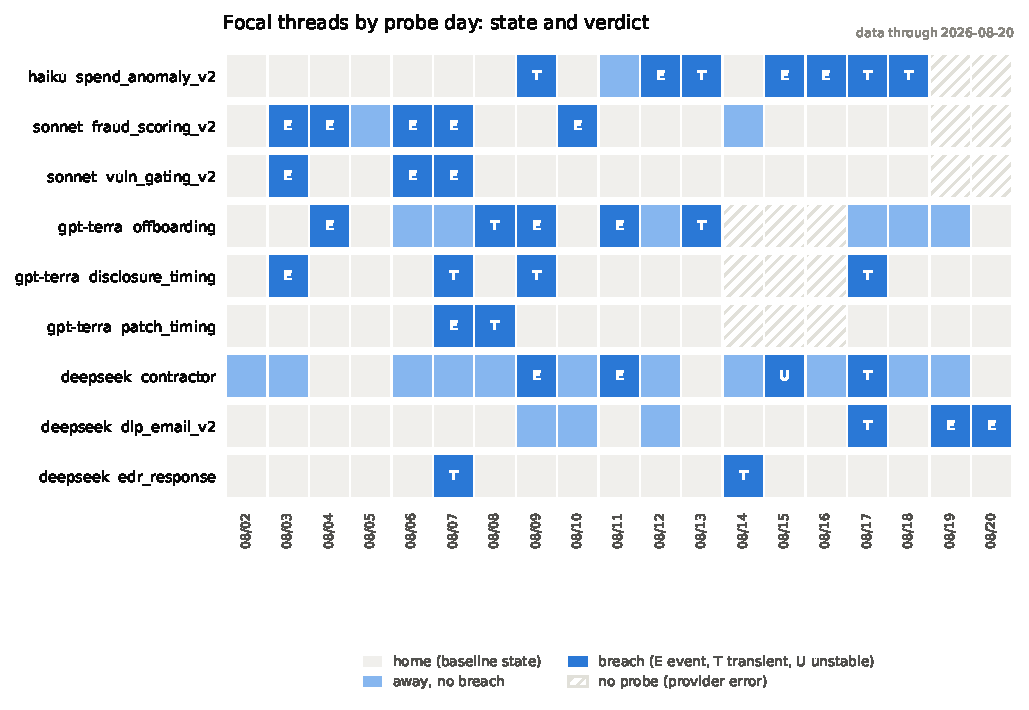
\includegraphics[width=\columnwidth]{f1_regime_map.pdf}
\caption{Regime map: focal threads by day, state timeline with
baseline, drifted, and breach marks per thread.
\freeze{placeholder render, data through 2026-08-20; regenerate
over the full window at the data freeze}}
\label{fig:regime}
\end{figure}

\begin{figure}[t]
\centering
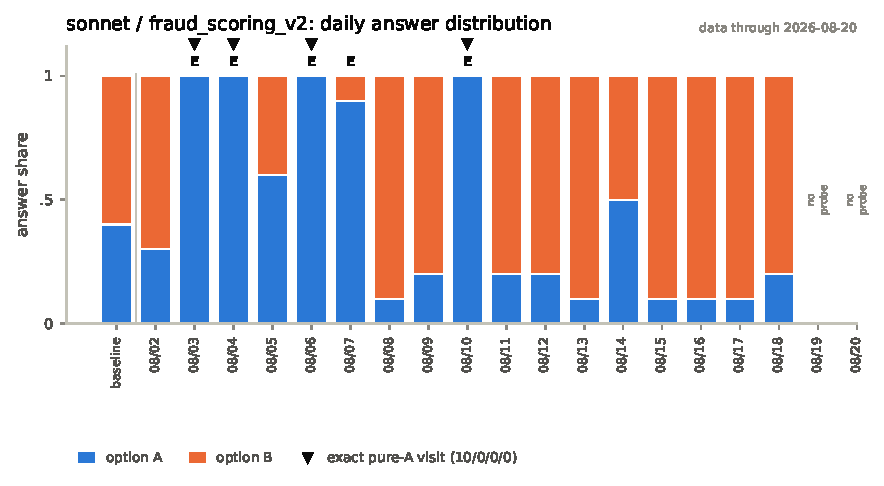
\includegraphics[width=\columnwidth]{f2_recurrence_strip.pdf}
\caption{Exact recurrence strip: the fraud-scoring item's daily
distributions as stacked bars, with the identical pure-A visits
annotated. \freeze{placeholder render, data through 2026-08-20;
regenerate at the data freeze}}
\label{fig:recurrence}
\end{figure}

\begin{figure}[t]
\centering
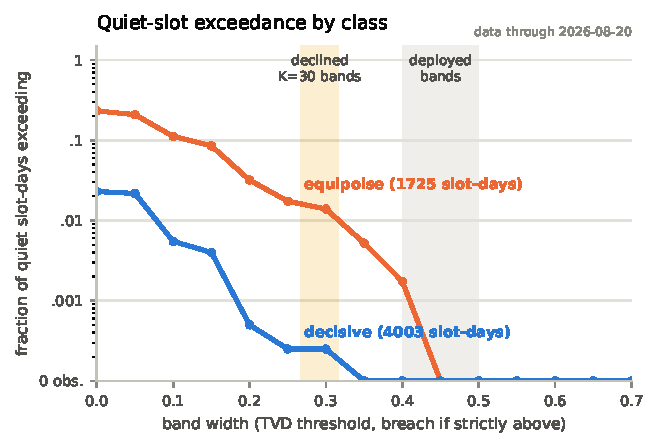
\includegraphics[width=\columnwidth]{f3_false_alarm_curve.pdf}
\caption{False-alarm curve: empirical quiet-slot exceedance
against band width, with the deployed bands and the declined
$K=30$ bands marked. \freeze{placeholder render, data through
2026-08-20; regenerate at the data freeze}}
\label{fig:falsealarm}
\end{figure}

One vendor's model held a two-item joint state (unanimous terse A
on a fraud-scoring item; verbose 9--10 D on a vulnerability-gating
item), left it, and re-entered it \freeze{twice in seven days},
with entries arriving as same-day joint moves and exits staggering
across days. The fraud-scoring item visited the identical pure-A
distribution \freeze{four times (Aug 3, 4, 6, 10)}
(Fig.~\ref{fig:recurrence}). A second vendor's offboarding item
recurred at exact vectors \freeze{8/0/2/0 three times, 9/0/1/0
twice}. A third vendor's spend-anomaly item settled into an away
state at the identical vector \freeze{0/6/0/4, twice by Aug 13; the
episode continued past the window and resolved under a
pre-committed decision rule, reported in
Section~\ref{sec:stepchange}}. Dwell in a state is one to two daily
observations; the attractor states themselves persist for weeks.
The same-day rerun bounds within-state reversion: across the
window, probe-to-rerun gaps run \freeze{0.43 to 5.28} minutes
(median 2.4), and reruns reproduced the probe exactly on the
strongest events.

Under the frozen baselines these are not plausible draws. The
recurring pure-A state has per-run probability
\freeze{$5.5\times10^{-5}$}; the 10 D verbose state,
\freeze{$1.6\times10^{-14}$ per run, $2.5\times10^{-28}$ across a
probe-rerun pair}. The states are also not new: they are prior
observed states of the same items. That is what motivates calling
this oscillation rather than drift.

\subsubsection{The pre-committed step-change rule}
\label{sec:stepchange}

The rule, committed 2026-08-16 blind to the deciding data, resolved
the first episode as alternation on its first evaluated day (a home
visit on Aug 14). A second away run began Aug 15 and crossed the
pre-committed threshold on 2026-08-23: seven consecutive observed
away days, every one B-modal on the identical discrete vector or a
deeper excursion, and the rule designated the item a step-change
candidate with no judgment in the loop. The operator response was a
dual-reference re-baseline: the alarm reference moved to the new
state, the frozen original stayed preserved in the same record, and
a return criterion against the original was pre-registered before
any new-regime data accrued \freeze{report the return-watch
outcome; a return day revises the classification to slow
alternation, no return leaves the step change standing with a
stated day-count bound, and both branches are dated commits}.

\subsection{The movement concentrates where judgment is contested}
\label{sec:concentration}

Every breach the monitor has recorded is an equipoise item.
\freeze{29 of 29} breach entries across \freeze{12} days landed on
designed-equipoise slots; the decisive class produced zero
exceedances in \freeze{2,700} slot-day observations. The honest
null share for the equipoise class is 0.381 of breach mass (not the
0.338 uniform share; equipoise bands sit differently), and the
concentration survives that weighting: \freeze{P(all-equipoise)
$7.3\times10^{-13}$ at entry level, $3.6\times10^{-6}$ on distinct
slots}.

The claim needs its ceiling stated. At $K=10$ the bands sit near
TVD 0.4 regardless of item distribution, so a breach needs roughly
four of ten samples to change category. Decisive items sit
unanimous at baseline; registering movement there requires close to
an outright answer flip. Decisive silence is an instrument ceiling,
not demonstrated stability. The defensible claim is that detectable
movement lives on contested judgment, and clear-cut behavior stayed
frozen at the resolution this instrument has.

\subsection{Structure against the honest null}
\label{sec:structure}

The breach count alone is weak evidence, and I will say so before
leaning elsewhere: \freeze{29 observed against 19.7 expected under
the smoothed null, $p = 0.029$}. What the null cannot produce is
the structure. Chance breaches spread across slots; the observed
entries pile onto repeat threads. \freeze{five slots carry three or
more breaches each, against 0.0101 expected slots at that depth,
$P = 8.0\times10^{-13}$.} Direction is structured too, and it
splits the threads into two morphologies. Every oscillator thread
moved toward the same option every time it moved \freeze{6 of 6 at
the drafting record, against 0.008 expected same-direction threads;
tails in Table~\ref{tab:structure}}. The one repeat thread that is
not direction-stable is not an oscillator at all: deepseek's
contractor-access item breached toward three different options
across four entries and carries the record's only UNSTABLE verdict,
a same-day rerun matching neither probe nor baseline. That thread
is a diffuse wander, not a two-state flip, and the two morphologies
are kept distinct wherever drift is counted
(\texttt{quiet\_slot\_decomposition.py}, part 3). Slots within a
model-day share a scaffold and are not independent; the recurrence
statistics are computed per-slot across days, where the sharing
argument does not apply, and the caveat is stated wherever the
numbers are.

\begin{table}[t]
\caption{Breach structure against the exact no-drift null.
\freeze{placeholder render, window 2026-08-02 to 2026-08-20, 19
probe days; regenerate at the data freeze}. Null: exact enumeration
under the smoothed baselines; the count row is deliberately weak
and reported first. Slots within a model-day share a scaffold and
are not independent; per-slot recurrence rows are computed across
days, where the sharing argument does not apply.}
\label{tab:structure}
\centering
\scriptsize
\setlength{\tabcolsep}{3pt}
\resizebox{\columnwidth}{!}{%
\begin{tabular}{lccc}
\hline
quantity & observed & expected (null) & $P(\geq \text{obs.})$ \\
\hline
breach entries & 43 & 31.206 & 0.02566 \\
distinct breached slots & 17 & 29.81 & \\
slots with $\geq$2 breaches & 9 & 1.3550 & $1.133\times10^{-5}$ \\
slots with $\geq$3 breaches & 7 & 0.042969 & $4.407\times10^{-14}$ \\
slots with $\geq$5 breaches & 3 & $2.41\times10^{-5}$ &
  $2.136\times10^{-15}$ \\
equipoise share of entries & 43 of 43 & null mass 0.38149 &
  $1.009\times10^{-18}$ \\
equipoise share, distinct slots & 17 of 17 & &
  $7.678\times10^{-8}$ \\
unidirectional $\geq$3-threads & 6 of 7 & 0.007581 &
  tail at 6: $2.131\times10^{-16}$ \\
unidirectional $\geq$5-threads & 3 of 3 & $1.67\times10^{-6}$ &
  tail at 3: $6.353\times10^{-19}$ \\
\hline
\end{tabular}%
}
\end{table}

\subsection{Detection without attribution}
\label{sec:attribution}

Behavior moved. Nothing else did. Across \freeze{41,090} rows,
every serving covariate visible from outside held constant: the
echoed model id never changed, reasoning flags were constant per
model, and no infrastructure field co-varied with any breach. The
EVENT label itself is weaker than designed and I demote it
honestly: the same-day rerun certifies persistence over \freeze{0.4
to 5.3} minutes, not the twenty the design assumed, and under a
serving-state correlation model the EVENT/TRANSIENT split carries
\freeze{$p = 0.68$} of discriminating power. The persistence
evidence is not the rerun. It is cross-day recurrence of exact
states.

The asymmetry is the operational point. A customer-side monitor can
say ``this model is not behaving as it did when qualified,'' with
dated, reproducible evidence. It cannot say why, and no amount of
black-box observation fixes that \cite{casper,cai}. The monitor's
product is a dated evidence trail, not a diagnosis.

\subsection{Temporal phenotypes}
\label{sec:phenotypes}

\begin{figure}[t]
\centering
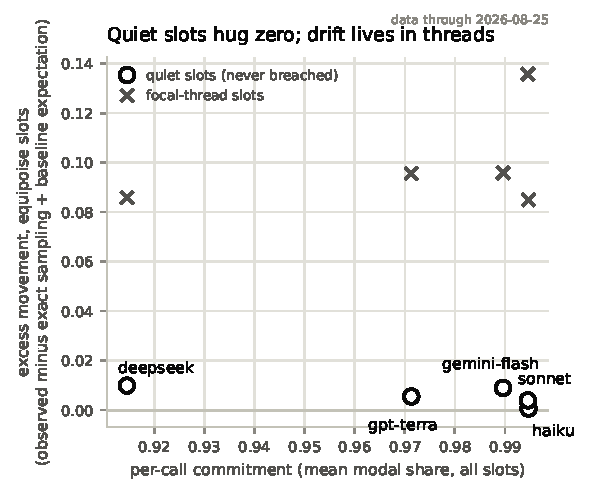
\includegraphics[width=\columnwidth]{f4_phenotype_grid.pdf}
\caption{Phenotype grid: per-call commitment against excess
movement, quiet and thread slots split per model; quiet slots hug
zero on all five. \freeze{placeholder render, data through
2026-08-20; regenerate at the data freeze}}
\label{fig:phenotype}
\end{figure}

Where drift does not live settles what per-call behavior means
(Fig.~\ref{fig:phenotype}). Outside the focal threads, no model
moves: on quiet equipoise slots, mean observed TVD sits within
\freeze{+0.009} of the exact expectation under a stationary
baseline, on all five models, once the expectation charges for
probe sampling and baseline estimation noise together. That holds
while per-call spread varies widely (mean modal share \freeze{0.92
to 0.99} across vendors). Ambient drift is zero at this
instrument's resolution; every detected movement belongs to a
named, recurring thread.

The phenotypes are therefore two axes that do not reduce to each
other: how a model answers (per-call commitment) and how it moves
when it moves (thread morphology). The Claude models and gpt are
commit-and-flip: near-deterministic per call, threads that are
discrete oscillations with exact state recurrence, entries
unidirectional every time. Deepseek is honest noise: the widest
per-call spread in the roster, quiet slots fully explained by
sampling arithmetic, and the record's only diffuse-wander thread in
its contractor item (its dlp thread is discrete, so the wander is a
thread property, not a vendor property). Gemini sat near-frozen
through the window \freeze{two transient breaches}. Per-call
determinism is not temporal stability, and the most
confident-looking style is the least snapshot-auditable.

Format rides along as an independent observable. On the
vulnerability-gating item, answer state and response format flip in
lockstep \freeze{148 of 150 samples}: terse 9-character rows in one
state, 766 to 1,421 character reasoned rows in the other. The
fraud-scoring item flips with zero length change. Format is a
serving-state signal the parsed-letter statistic only sees when the
letter moves; it is captured per row and reported descriptively.

\section{What the instrument got wrong}

The CFP asks for honest failure. Five items, each a dated commit in
the public record, each load-bearing for someone building the same
thing.

\begin{enumerate}
\renewcommand{\theenumi}{\alph{enumi}}
\renewcommand{\labelenumi}{(\theenumi)}
\item The false-alarm arithmetic was wrong first. Working analysis
  estimated 3.4 chance breaches per day by treating p99 as an exact
  exceedance rate; on a discrete statistic at $K=10$ it is not.
  Exact enumeration corrected it to 1.64 (smoothed truth) and 0.05
  (empirical truth), and the correction is the citable number.
\item A sensitivity upgrade was approved, built, and declined the
  same day. $K=30$ narrows bands from roughly 0.40 to \freeze{0.267
  to 0.317}; the between-day variance the bands never modeled sits
  at \freeze{p99 = 0.35} on equipoise items, above the proposed
  bands. Shipping it would have manufactured \freeze{1.5 to 2.5}
  false alarms per day. Two weeks of accumulated cross-day data
  vindicated the decline empirically.
\item The frozen baseline can be the anomaly. \freeze{82 of 115}
  equipoise slots were unanimous at baseline, on items designed to
  split. For those slots the monitor may have enshrined an
  excursion as the reference and then alarmed on movement toward
  designed behavior. The instrument therefore says ``changed,''
  never ``degraded''; the sign of change is not identified.
\item EVENT certifies minutes, not the roughly twenty the design
  assumed. Measured probe-to-rerun gaps run \freeze{0.43 to 5.28}
  minutes. The label was demoted in the analysis rather than
  defended.
\item The first version of this paper's phenotype figure repeated
  the baseline error in miniature. Its expected-movement term
  treated the frozen $n=20$ baseline as exact, which charges the
  widest-distribution vendor for its own sampling spread, and the
  figure misread honest noise as drift. The corrected expectation
  propagates baseline noise exactly; mistake and correction are
  same-day dated commits.
\end{enumerate}

\section{Operational guidance}

For a team running judgment-layer automation on a frontier API, the
numbers above convert to practice.

Split the bank by class and band accordingly. Decisive items are
near-noiseless (\freeze{zero exceedances above 0.20 in 2,700
slot-days}): their bands can tighten to 0.25 and monitoring there
is essentially free sensitivity. Equipoise bands cannot narrow at
$K=10$: between-day spread does not shrink with $K$ (\freeze{sqrt-K
scaling measured wrong for the equipoise class}), so they stay at
0.40 or above and their alarms are read as regime signals, not
degradation.

Treat snapshot evaluation as day-certification. A passed eval
certifies the day it ran. Period assurance requires a monitor in
the loop, and the monitor defines the compensating control: route
flagged periods to secondary review, gate automated decisions
qualified against prior behavior, and write the observable into
vendor contracts (distribution stability on a pinned bank), not the
cause, which no customer can observe.

Know what the tool cannot do. Detection tells you when to stop
trusting your own automation. It does not tell you whom to blame,
and procurement or contract language that assumes attribution from
outside the API is writing a check the measurement cannot cash.

\section{Related work}

Log-probability and token-level API change detection
\cite{chauvin-a,chauvin-b} targets the same problem with
instruments that require persistence: multi-day filters and one-way
changepoints. The oscillation class documented here is discarded by
those designs by construction; a state that reverts within days
never survives a four-day persistence filter. The instruments are
complementary, and the reversible class needed one that keeps it.
Daily and weekly periodicity in LLM performance \cite{tschisgale}
is the continuous cousin of the discrete recurrence here.
Longitudinal behavioral change on major APIs is established at
month scale \cite{chen}; this work moves the resolution to days and
adds exact state recurrence. The attribution ceiling is structural,
not a limitation of effort: black-box access does not support
causal attribution of serving-stack change \cite{casper}, and
software-only verification of served models remains brittle
\cite{cai}. Boundary-item drift sensing predates LLMs:
margin-density drift detection placed its sensors at the decision
boundary \cite{md3}, the same design choice the equipoise class
makes here. Vendor-side ground truth that serving changes ship,
stick per-user, and evade vendor evals comes from a published
postmortem \cite{anthropic-postmortem}; the numerics mechanism for
silent behavioral variation is documented in
\cite{thinking-machines}.

\section{Limitations and reproducibility}

One bank, five models, one scaffold, \freeze{N} days. The
phenotypes are observed styles, not vendor properties. Slots within
a model-day share a scaffold; day-level counts are overdispersed
and the per-slot recurrence statistics carry the independence
caveat stated in Section~\ref{sec:structure}. The detection floor
at $K=10$ is roughly a four-of-ten answer shift, so sub-floor
movement is invisible and decisive-class stability is bounded, not
proven. The strict inequality at the band is load-bearing: moving
to greater-or-equal raises null breach mass \freeze{4.8$\times$}.
Cost and cadence are modest by design; the instrument trades
sensitivity for a false-alarm budget an operator can actually
staff.

The full instrument is reproducible: item bank, baselines, bands,
seeds, verdict log, analysis scripts, and every correction cited
above as dated history. \pendingnote{Blind-review handling per the
handoff: decide before submission. Default if the organizers do not
object: ``public artifact, link on acceptance''; otherwise an
anonymized mirror for review. Do not cite the repository by name in
the submitted PDF.}

\bibliographystyle{IEEEtran}
\bibliography{references}

\end{document}
